% !TEX root = report.tex

\section{Processing Pipeline}
\label{sec:processing_architecture}

High level descripion of the processing flow:

Throughout the report: extract Spectrograms, classify image.

Some experiments extract only the loudest section of the inputs.

Test against a stream of sounds.

\section{Signals and Features}
\label{sec:model}

\subsection{Input Datasets}

\subsubsection{Google Dataset}

% Measurement setup, data preprocess (describe the google dataset)

The Speech Commands datasets \cite{warden2018speech} (GSCD), provides thousands
of one second recording of $35$ different words. The recordings are mainly of
volounteers, who used their own device to record the words in a closed room
wherever they happened to be (not in a studio setting). Ideally each volounteer
only recorded the $135$ requested utterances once, so the dataset provides good
variability of voices.
The utterances have a duration of one second.
To more precisely align the recorded clips, the audio was acquired for $1.5$
seconds and the $1$ second clip that contained the highest overrall volume was
extracted.
Several background noise recording are included as well.
The full dataset includes $105829$ utterances of $35$ words, saved in
\textit{.wav} format at $16$ KHz rate.
The dataset is released under the Creative Commons Attribution $4.0$
International (CC~BY~$4.0$) License \cite{ccby4}.
The dataset ships with a function to split the data in train, validation and
test folds, as well as two example lists of validation data ($9981$ utterances)
and test data ($11005$ utterances).
Throughout the experiments, those lists were used.
% MAYBE both for the practicality of having them ready, but also to keep with
% the spirit of the dataset as a tool to enable meaningf

The Speech Commands dataset was preprocessed, extracting for each $1$ second
utterance the loudest $0.5$ second section, using a simple analysis of the
signal's power.

TODO: comparison of 1 sec clip and loudest section, with spectrograms

\subsubsection{Free Spoken Digit Dataset}

As a test dataset, the Free Spoken Digit Dataset was used
\cite{zohar_jackson_2018_1342401}.
The current version of the dataset contains $3000$ recordings made by $6$
speakers, $50$ utterances of each digit per speaker.
Each utterance is saved in \textit{.wav} format at $8$ KHz rate.
The dataset is released under the Creative Commons 
Attribution-ShareAlike $4.0$ International (CC~BY-SA~$4.0$)
License \cite{ccbysa4}.
This dataset was only used after all hyper-parameters were tuned, to evaluate
the performances on fresh data.

\subsubsection{LibriTTS}

To evaluate the model in a streaming setting, a section of LibriTTS was used
\cite{zen2019libritts}.
This dataset contains approximately $585$ hours of English speech, aligned at
sentence level.
Both original and normalized text is included (e.g. ``June $9$, $1872$'' is
converted in ``june ninth eighteen seventy two''), and each sentence is saved
in \textit{.wav} format at $24$ KHz rate.
Metadata information regarding the speakers, the books and the chapters is
available, but was not needed in this project.
The dataset is released under the Creative Commons Attribution $4.0$
International (CC~BY~$4.0$) License \cite{ccby4}.

TODO: split in sentences that have or not the words.

\subsection{Tasks definition}

Smaller tasks were used to evaluate the performance of the various
architectures, and to perform the hyper-parameter search.
The set of tasks and the identifier key for GSCD is as follows:
Two $4$ words task are composed by the words
\texttt{f1}: [\texttt{happy}, \texttt{learn}, \texttt{wow}, \texttt{visual}],
\texttt{f2}: [\texttt{backward}, \texttt{eight}, \texttt{go}, \texttt{yes}].
A $6$ words task contains the direction words:
\texttt{dir}: [\texttt{up}, \texttt{down}, \texttt{forward}, \texttt{backward},
\texttt{left}, \texttt{right}]
Two $10$ words task contains the number utterances:
\texttt{num}: [\texttt{zero}, \texttt{one}, \texttt{two}, \texttt{three}, \texttt{four},
\texttt{five}, \texttt{six}, \texttt{seven}, \texttt{eight}, \texttt{nine}]
and the words from a Kaggle competition aimed at solving this task:
\texttt{k1}: [\texttt{yes}, \texttt{no}, \texttt{up}, \texttt{down}, \texttt{left},
\texttt{right}, \texttt{on}, \texttt{off}, \texttt{stop}, \texttt{go}].
A $20$ words task (\texttt{w2}) is composed by the numbers and the Kaggle list, and
a $35$ words task (\texttt{all}) uses the entire dataset.

For FSDD, each number is prefixed with \texttt{fsdd\_}, and the set of words is
referred as \texttt{fsdd\_num}.

For LibriTTS, in addition to these categories, another word label is added:
\texttt{\_other\_ltts}. This category is used to discriminate a conversation
that does not contain the $35$ command words.
Each task for GSCD is expanded by adding this category, and is referred as
\texttt{LT\_\{task\_key\}}.

For the shortened utterances extracted from GSCD, each word is prefixed with
\texttt{loudest\_}, and
the set of words is referred as
\texttt{\{task\_key\}\_LS}.

\subsection{Mel spectrogram and Mel-frequency Cepstral Coefficients}

The audio data in the dataset is available as a vector of amplitudes over time,
sampled at $16$ KHz. In this representation, the classification task is quite
hard.
The Fourier transform allows to convert a signal from the time domain into the
frequency domain. The result is called spectrum of the signal. This transform
is efficiently computed using the Fast Fourier Transform algorithm.

The short-time Fourier transform accounts for variations of the content of an
audio signal over time. Instead of computing the FFT of the entire signal, the
FFT is computed on overlapping windowed segments of the signal: each window has
length \texttt{n\_fft} and the next window is extracted after
\texttt{hop\_length} samples.
The results of the FFT in each window are stacked to obtain the spectrogram.

The human ear does not perceive frequencies on a linear scale: the difference
between $200$ and $400$ Hz is very marked, whereas two notes at $8000$ and
$8200$ Hz are almost indistinguishable. The mel scale, proposed by Stevens,
Volkmann, and Newmann \cite{melscale1937}, introduces a unit of pitch built in
such a way that equal distances on the scale sound equally distant to the human
listener.
The mel spectrogram is a spectrogram where the frequencies are converted to the
mel scale. To do so, a Mel spaced filterbank is generated (a 10 filters version
is shown in \fig{fig:mel10_filterbank}) and the FFT results are multiplied with
a dot product with each filter, obtaining \texttt{n\_mel} values for each
timestep.

\begin{figure}[t!]
    \centering
    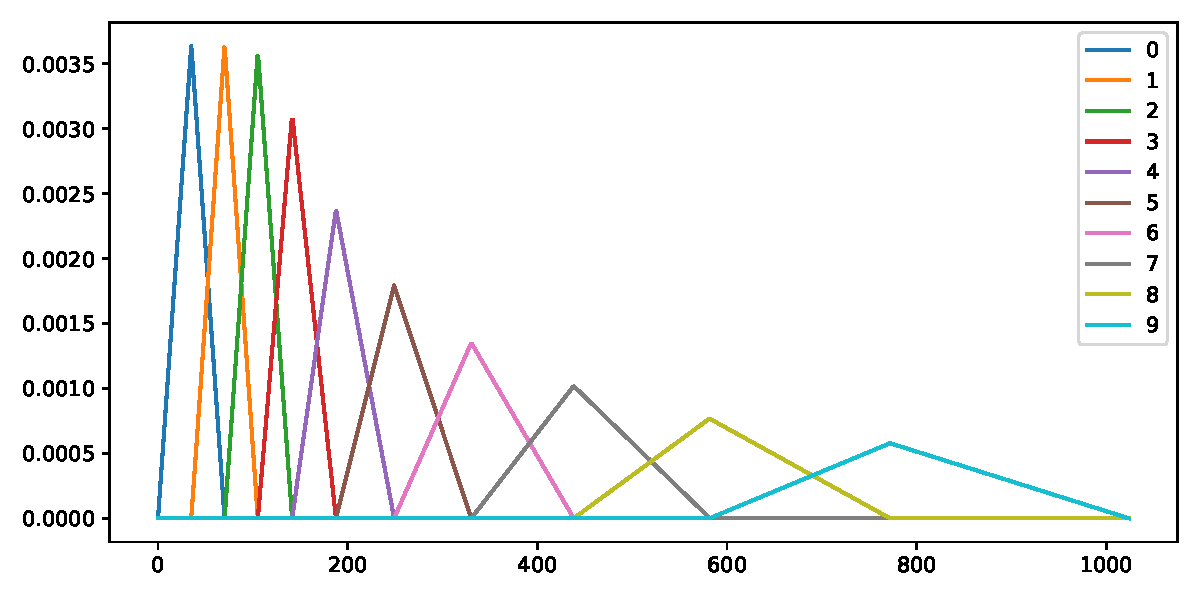
\includegraphics[width=0.9\linewidth]{mel10_filterbank.pdf}
    \caption{An example of a 10 filters Mel filterbank}
    \label{fig:mel10_filterbank}
\end{figure}

The resulting coefficients are highly correlated: the Discrete Cosine Transform
can be applied to decorrelate the filter bank coefficients and obtain a
compressed representation.
The results are the Mel-frequency Cepstral Coefficients.

The spectrograms were obtained using the \texttt{librosa} library
\cite{brian_mcfee_2020_3955228}.
The values used to generate the mel spectrograms are listed in
\tab{tab:mel_values}.
The values used to generate the mel frequency cepstral coefficients are listed
in \tab{tab:mfcc_values}.
An example waveform for the word ``happy'' and the relative spectrograms are
shown in \fig{fig:happy_specs}.

Some of the architectures that were tested require a square image as input,
with three color channels.
To obtain them, some spectrogams were purposefully generated with parameters
that created a square result, others, shaped like a half square, were
concatenated, as shown in the ``melc1'' spectrogram in
\fig{fig:happy_mel01_mel04_mel06_melc1_specs}.
Three square spectrogams are then stacked depthwise to obtain a valid three
channel image.
The values used to compose the spectrogams are listed in \tab{tab:compose_values}.
The values used to stack the spectrogams are listed in \tab{tab:ch3_values}.

\begin{figure}[t!]
    \centering
    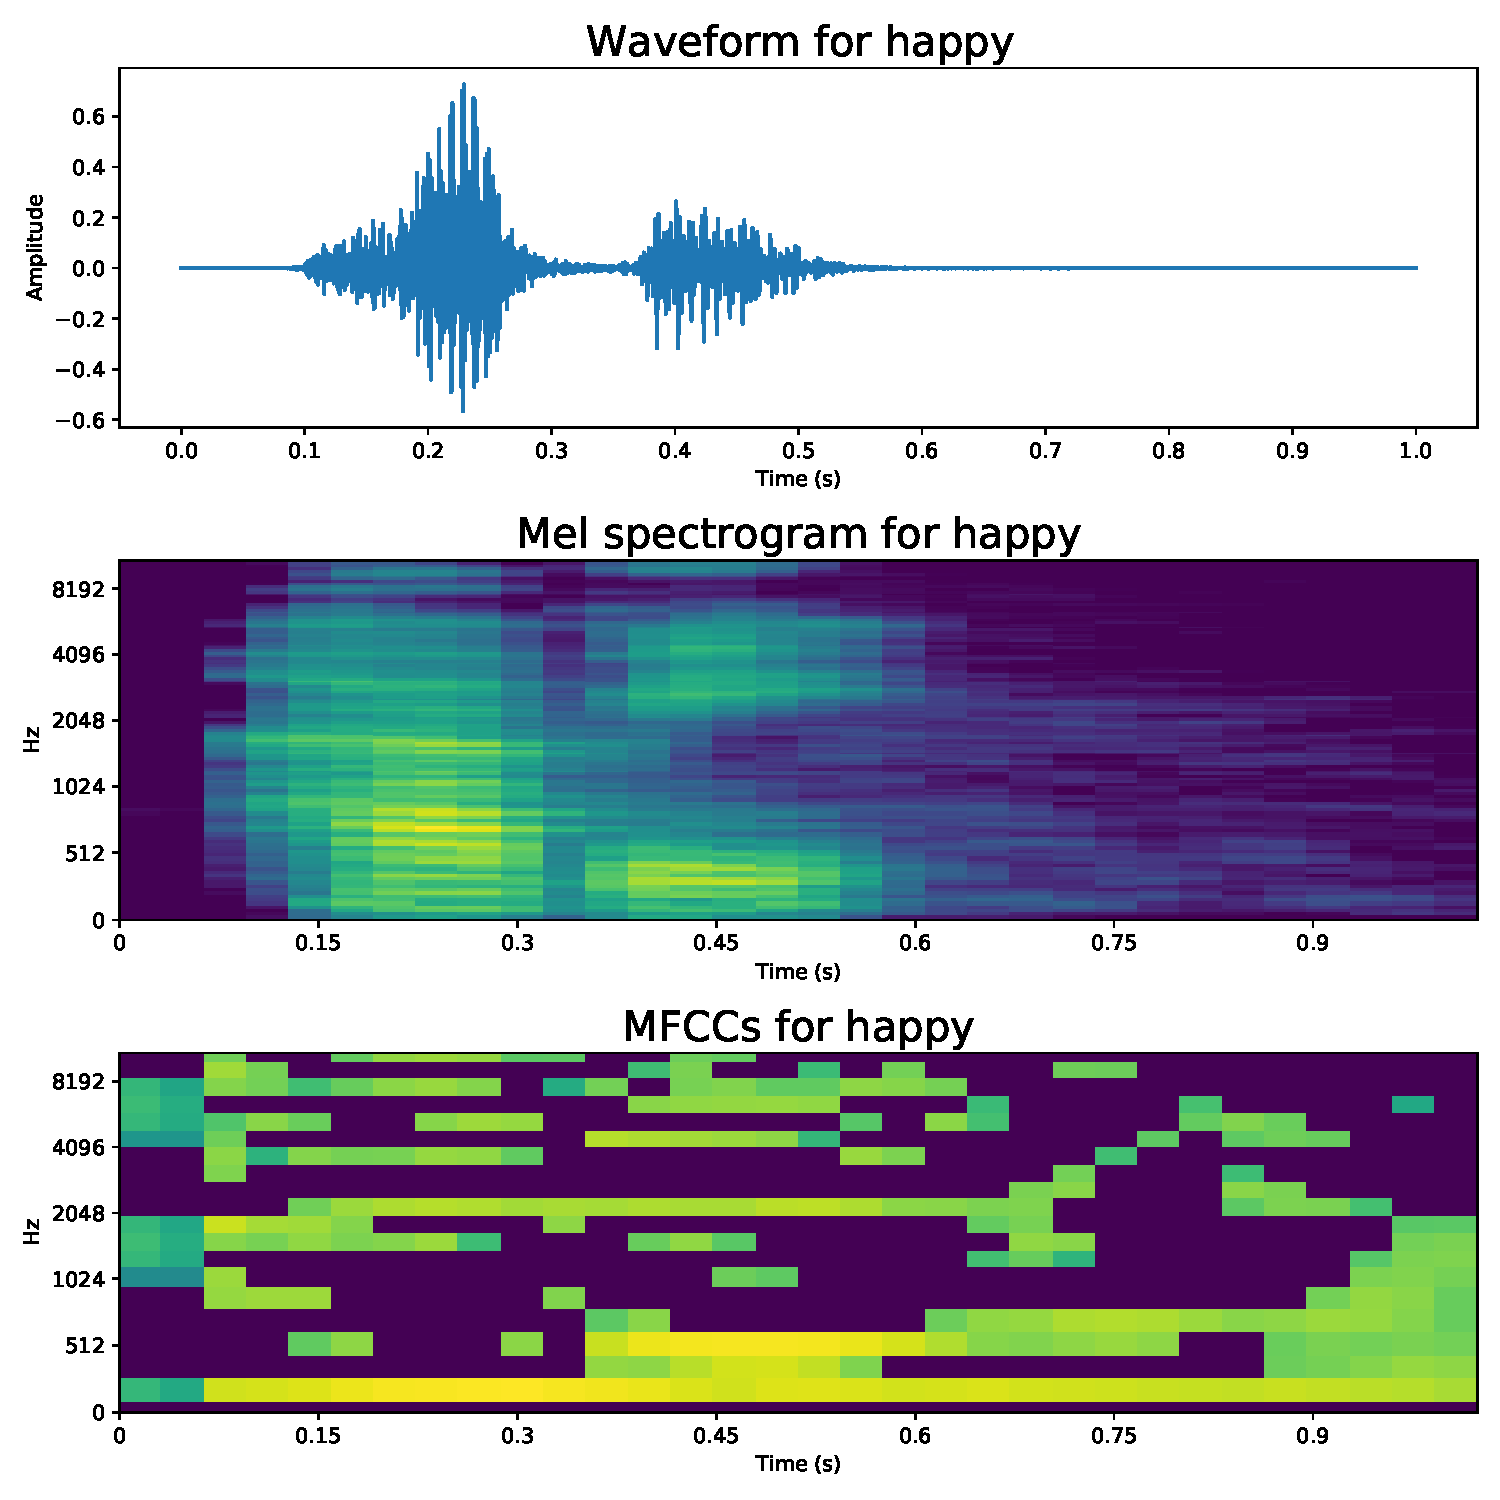
\includegraphics[width=0.9\linewidth]{happy_specs.pdf}
    \caption{
    Waveform and spectrograms for the word happy. Note that the y axis of the
spectrograms are labeled as Hz, but this is only to read more easily the plot
and understand to which frequencies the important bins correspond to. }%
    \label{fig:happy_specs}
\end{figure}

\begin{figure}[t!]
    \centering
    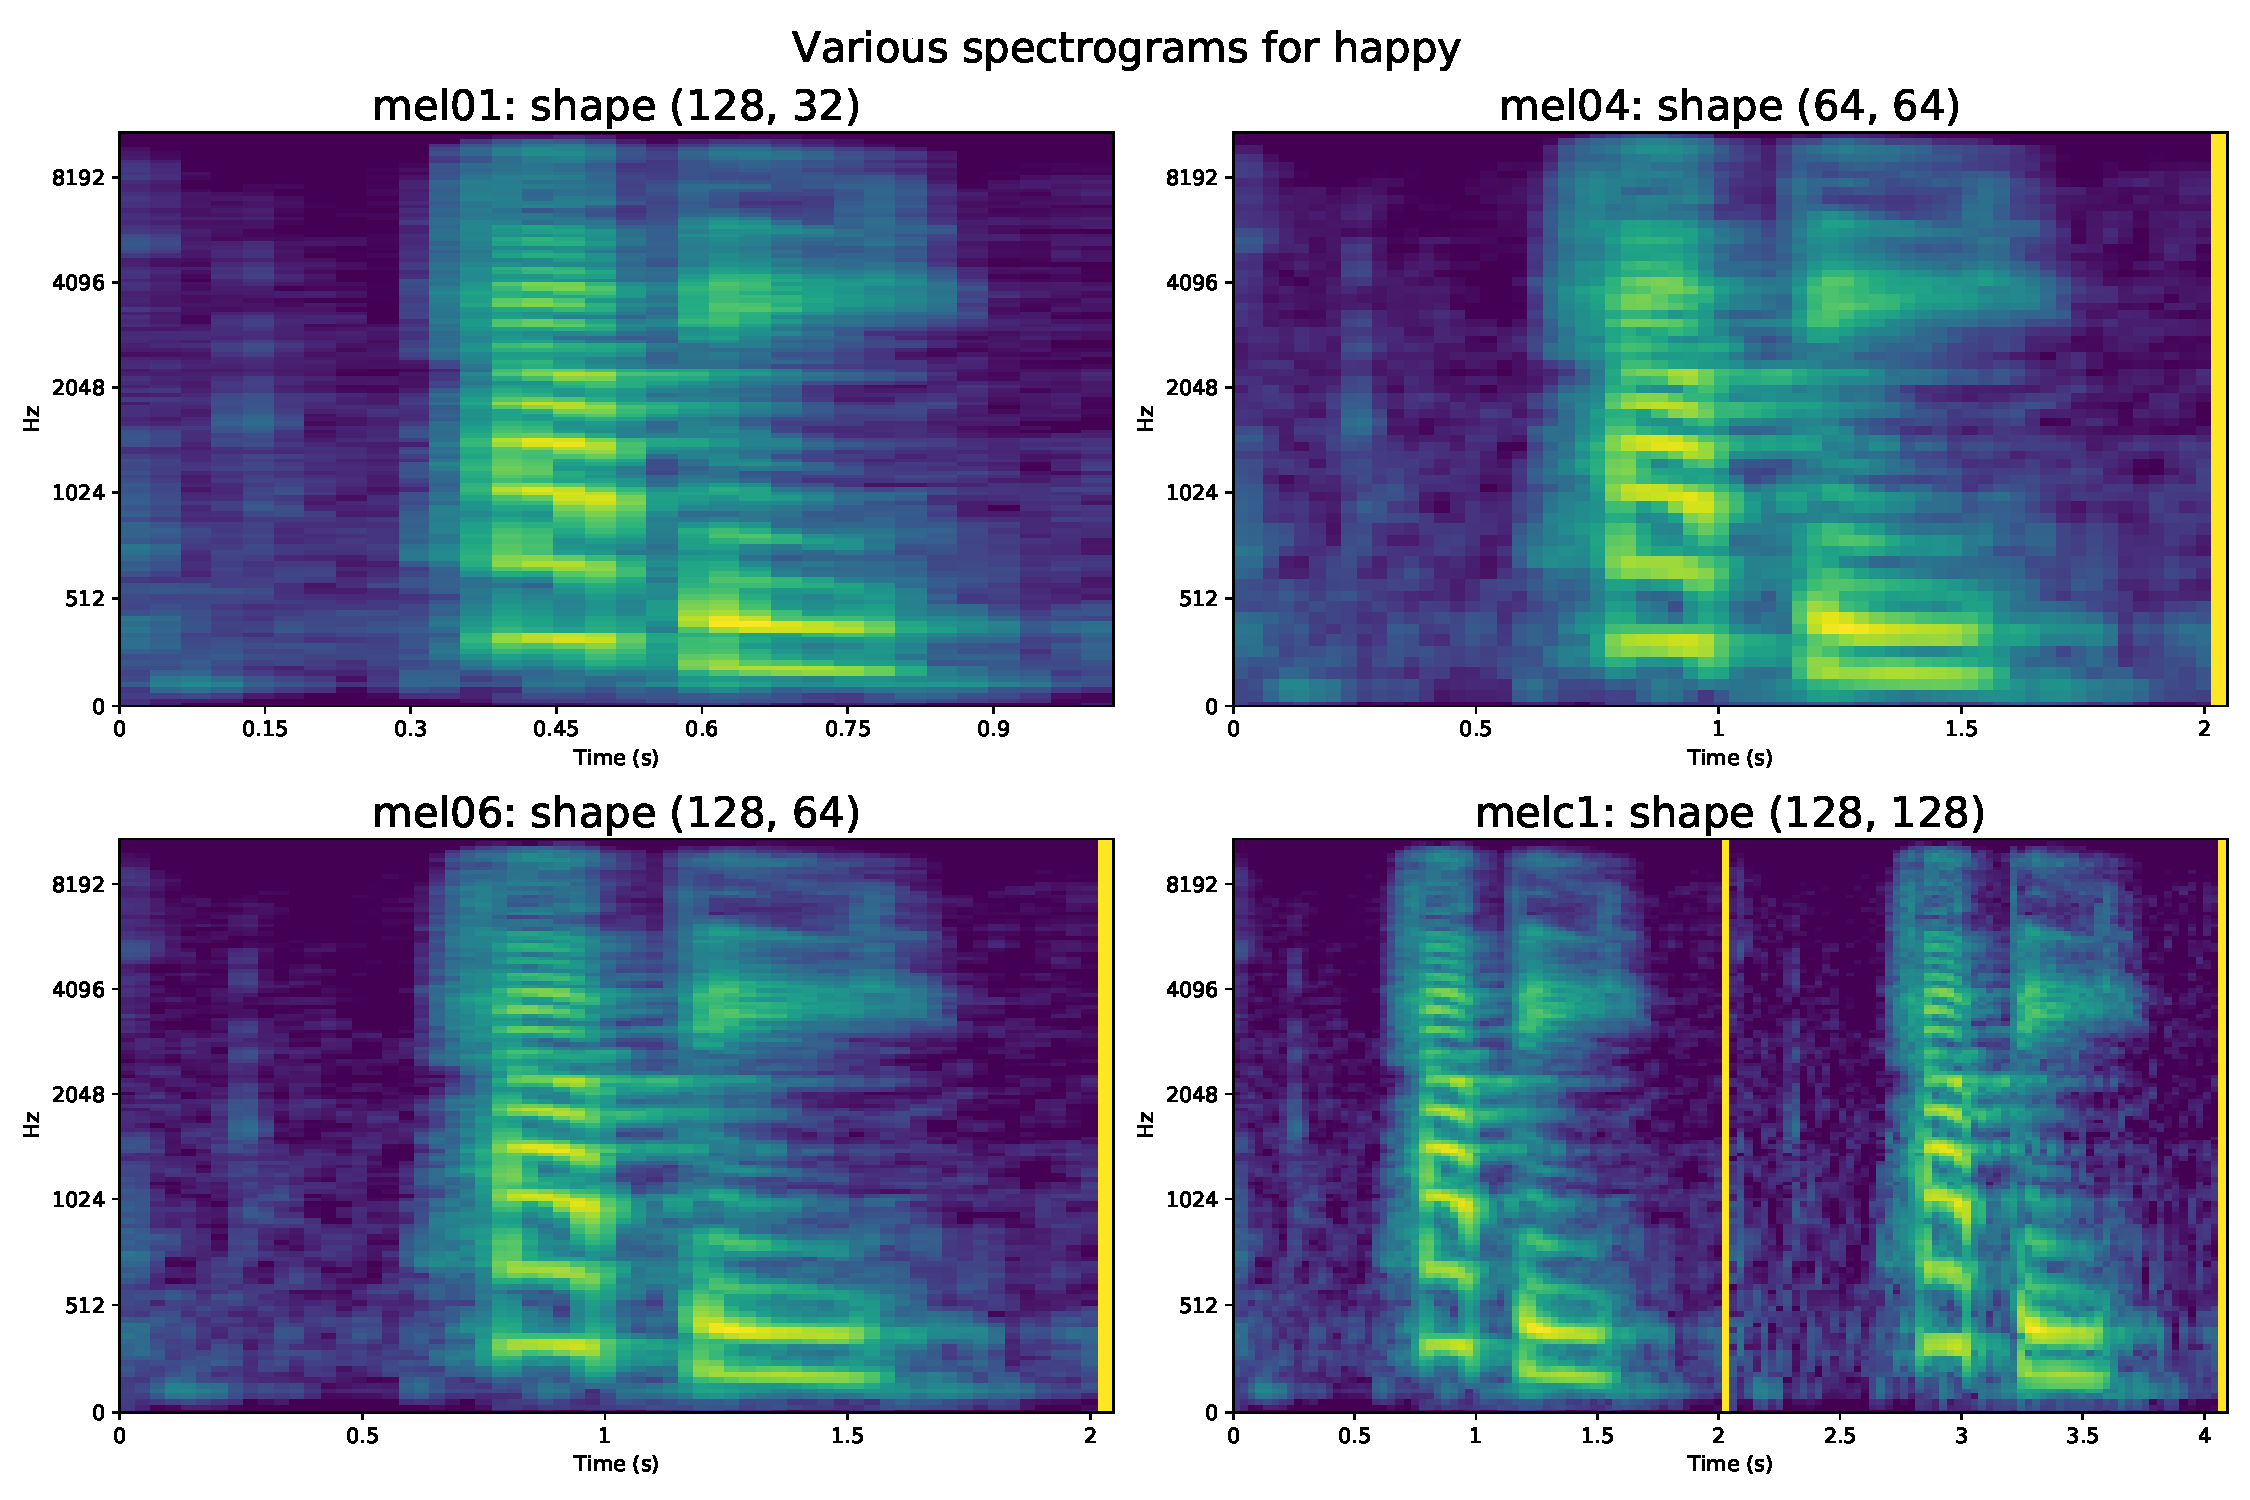
\includegraphics[width=0.9\linewidth]{happy_mel01_mel04_mel06_melc1_specs.pdf}
    \caption{Different spectrograms for the same word}%
    \label{fig:happy_mel01_mel04_mel06_melc1_specs}
\end{figure}

TODO: decision of preprocessing the data separately.

\subsection{Data augmentation}
\label{sec:data_augmentation}

Data augmentation is a technique to increase the amount of data available by
applying random, but meaningful, transformations to the data. This leads to a
noisier dataset, that should make the trained model more robust and less prone
to overfitting. The data was augmented both by modifying the waveform and the
spectrograms. An option to include the originals in the augmente dataset is
available.

\subsubsection{Time shift}

The waveform is shifted by a random amount of samples, controlled by the
parameter \texttt{max\_time\_shift}.

\subsubsection{Time stretch}

The waveform is stretched, making the sound slower or faster, controlled by the
parameter \texttt{stretch\_rate}.

\subsubsection{Spectrogram warp}

The spectrogram is warped using the \texttt{sparse\_image\_warp} function
available as a tensorflow addon.
A sequence of source landmarks is randomly selected within the image, and the
points are shifted by a random amount along both time and frequency axis. The
warp is controlled by the parameters \texttt{num\_landmarks},
\texttt{max\_warp\_time} and \texttt{max\_warp\_freq}.
The effect of warping an image is shown in \fig{fig:warp_grid}.

Several augmentations were performed, mostly focussing on the spectrogram
warping, along one or both time and frequency axis.
Values used to augment the dataset are listed in \tab{tab:aug_values}.

\begin{figure}[t!]
    \centering
    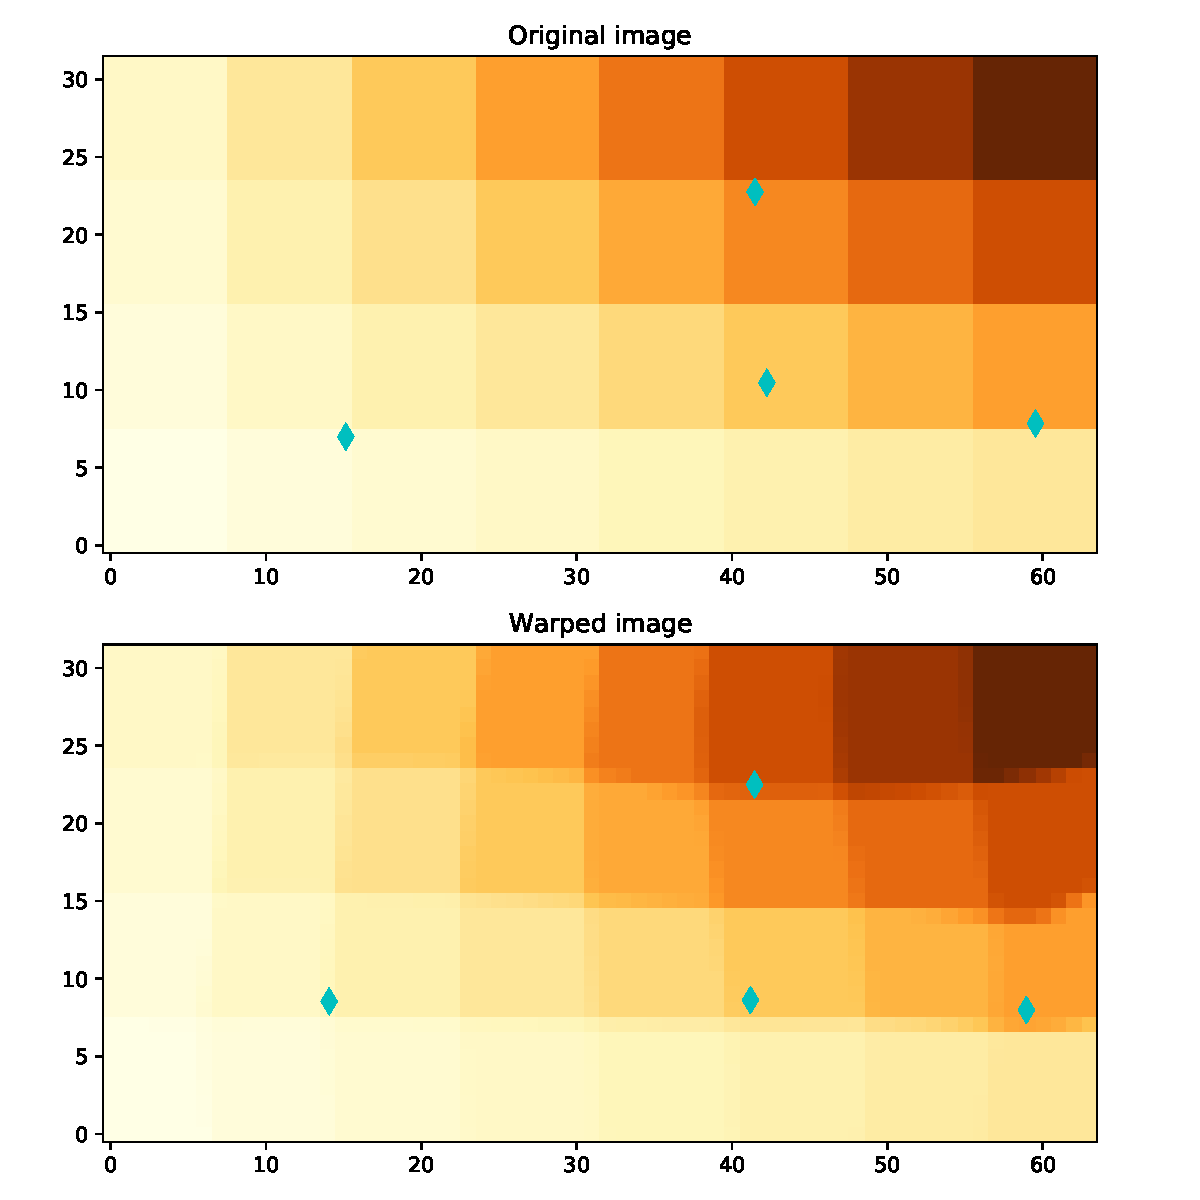
\includegraphics[width=0.9\linewidth]{warp_grid.pdf}
    \caption{
    The effects of \texttt{sparse\_image\_warp} on an image, with
\texttt{num\_landmarks} $=4$, \texttt{max\_warp\_time} $=2$ and
\texttt{max\_warp\_freq} $=2$. The diamonds show the source and destination
landmarks.}%
    \label{fig:warp_grid}
\end{figure}

\section{Learning Framework}
\label{sec:learning_framework}

% TODO: See Kumar Xception 4.4

The training was done using the tensorflow library \cite{tensorflow2015-whitepaper}.

% TODO: intro to this section.

Several training details can be adjusted to achieve optimal performance.
An overview of the parameters tweaked during the experiments is provided in
this section.

\subsection{Learning rate}

During the experiments, different values of learning rate and different
schedules were used:
% TODO: de novo?
% The details are described in this section.

\subsubsection{Finding optimal LR values}
\label{sec:lr_sweep}

For a model to learn, an optimizer computes the error gradient for the current
model using a batch of training samples, then uses the back-propagation
algorithm to update the weights of the model.
The learning rate controls how much the model weights are changed after each batch.
If the value is set too low, the model is not able to learn, and the loss does
not decrease at all.
If the value is set too high, the model changes too much after each batch,
which leads to quick variations in the loss and the model ultimately cannot
converge.

To find proper values for the learning rate, a technique that sweeps all
possible values was used \cite{PYISlearningsweep}.
The algorithm starts learning with an extremely low value for the learning rate
($1e-9$), then exponentially increases this value after each batch update. The
training continues until the learning rate reaches $1$ or the loss diverges too
much.
The loss value for each learning rate value is logged and the results are shown
in \fig{fig:LR_sweep_bs16_en15}.
From the plot the optimal range for the learning rate can be easily inferred:
the model started learning at $1e-5$ and the training started to diverge at
$1e-3$. The latter value can be chosen as initial learning rate and the former
to tune the learning rate decay.

% https://latexdraw.com/how-to-annotate-an-image-in-latex/
\begin{figure}[t!]
    \centering
    \begin{tikzpicture}
        \node[above right] (image) at (0,0) {
            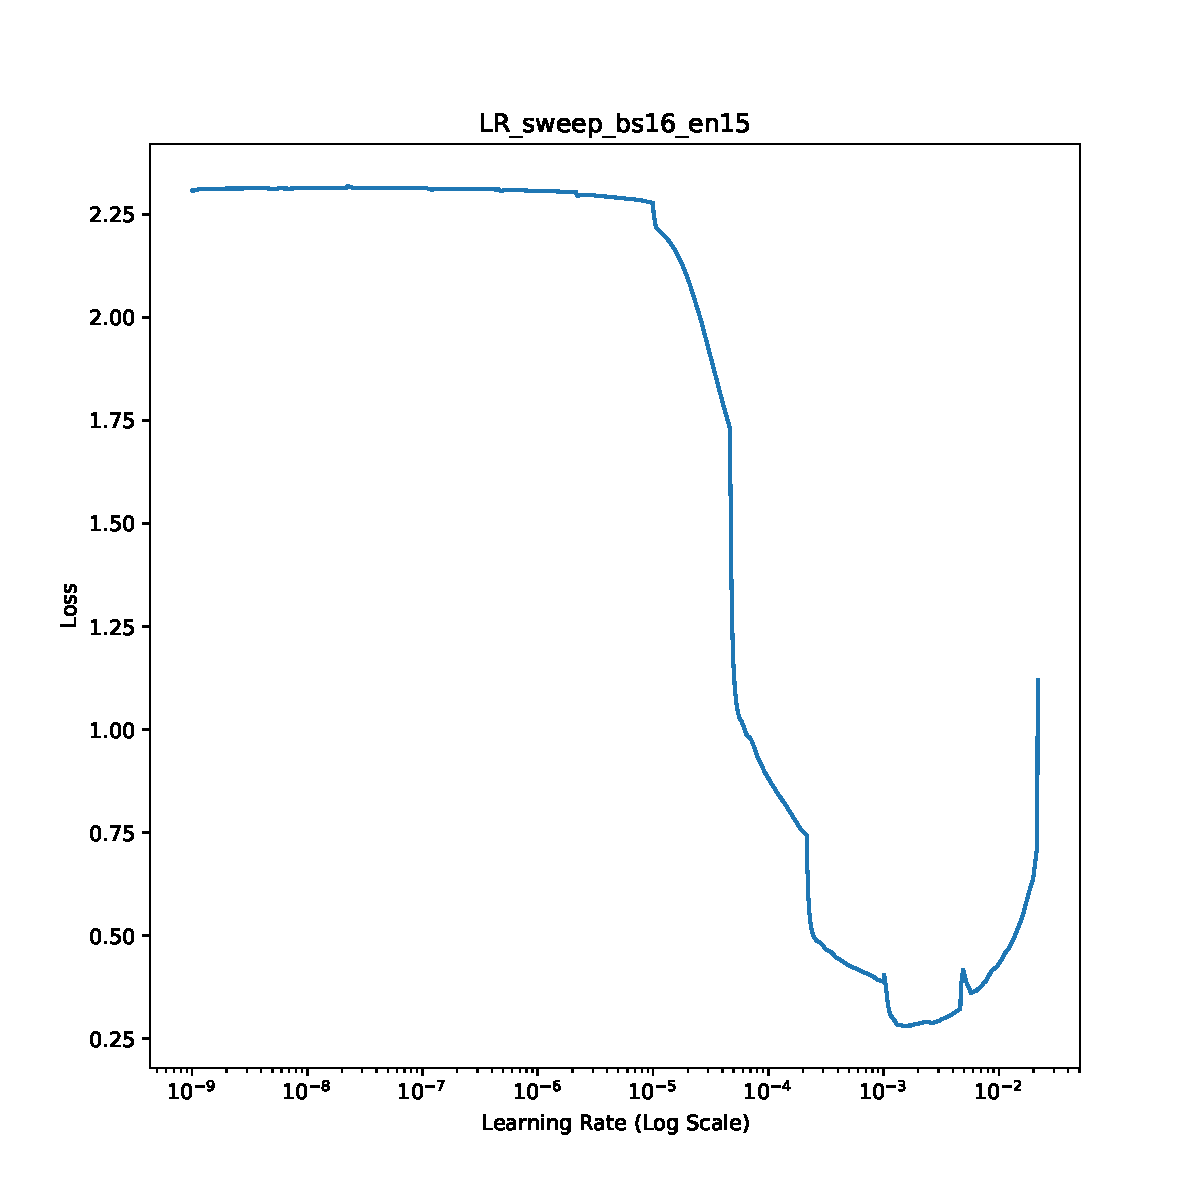
\includegraphics[width=0.9\linewidth]{LR_sweep_bs16_en15.pdf}
        };
        \draw[latex-, very thick,red] (4.3,6.4) -- ++(-1,-1.2)
            node[below, black, fill=white, text width=2.5cm, align=center]{
            \small The loss starts to drop at $1e-5$
        };
        \draw[latex-, very thick,red] (5.9,1.3) -- ++(-1.5,0.4)
            node[above left, black, fill=white, text width=2.5cm, align=center]{
            \small The loss starts to increase at $1e-3$
        };
    \end{tikzpicture}
    \caption{LR sweep with \texttt{batch\_size} 16, \texttt{epoch\_num} 15.}%
    \label{fig:LR_sweep_bs16_en15}
\end{figure}

\subsubsection{Learning rate schedules}

Different schedules for the learning rate can be used, to set a specific learning rate each epoch:

\paragraph{Fixed}

The simplest schedule consist in a constant function that keeps the value fixed
(e.g. \texttt{lr}$=1e-3$).
% , \texttt{lr}$=1e-4$).

\paragraph{Exponential decay}

The exponential decay schedule decreases the learning rate by a certain factor
each epoch. The shape of the decay is controlled by \texttt{initial\_lr},
\texttt{drop}, \texttt{epochs\_drop} and \texttt{min\_lr}:
\begin{equation}
    lr =
    \max \left\{ 
        min\_lr,
        initial\_lr * drop ^{ \frac{1 + epoch}{epochs\_drop} }
    \right\}
    .
    \label{eq:lr_smooth}
\end{equation}
The step version of this schedule drops the learning rate every
\texttt{epochs\_drop} epochs:
\begin{equation}
    lr =
    \max \left\{ 
        min\_lr,
        initial\_lr * drop ^{
            \left\lfloor 
                \frac{1 + epoch}{epochs\_drop}
            \right\rfloor
        }
    \right\}
    .
    \label{eq:lr_step}
\end{equation}
The two different schedules are compared in \fig{fig:lr_step_smooth}.
\begin{figure}[t!]
    \centering
    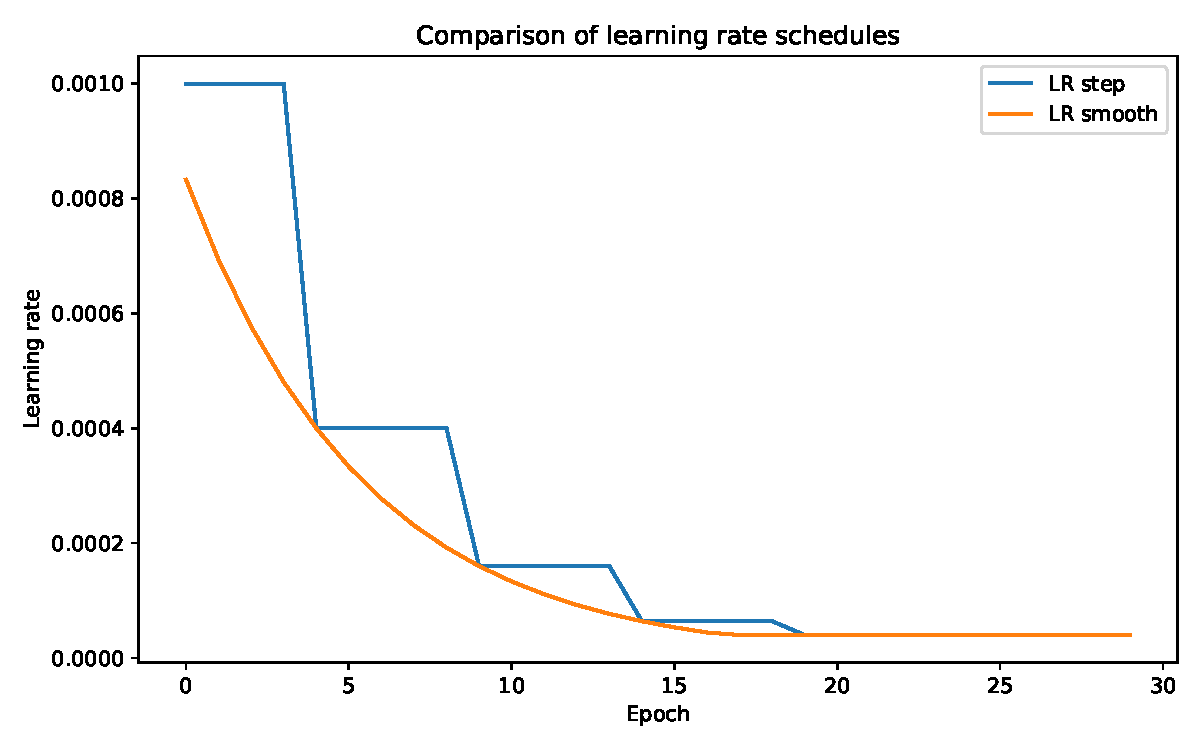
\includegraphics[width=0.9\linewidth]{lr_step_smooth.pdf}
    \caption{Learning rate schedules: exponential decay, step and smooth.
        Parameters:
        \texttt{initial\_lr} $=0.001$,
        \texttt{drop} $=0.4$,
        \texttt{epochs\_drop} $=5$,
        \texttt{min\_lr} $=4e-5$.
        The minimum value is reached at epoch $19$.}%
    \label{fig:lr_step_smooth}
\end{figure}

\paragraph{Cyclic}

One of the problem to solve when optimizing a function is avoiding local minima.
A low learning rate might not be sufficient to escape the area and descend
towards the global minimum.
A cyclic learning rate schedule \cite{smith2017cyclical} can solve this problem,
oscillating the learning rate cyclically between two values.
One implementation of this policy as a tensorflow callback is available on
GitHub \cite{bckenstlerCLR}.
An example of the \texttt{triangular2} policy is shown by
\fig{fig:cyclic_lr_example}: a sharp initial drop in loss can be seen, as the
learning rate covers the optimal range of values found by sweeping, as
described in \secref{sec:lr_sweep}. A small increase in loss corresponds to the
peak of the second cycle. Finally with the last two cycles the model converges.

\begin{figure}[t!]
    \centering
    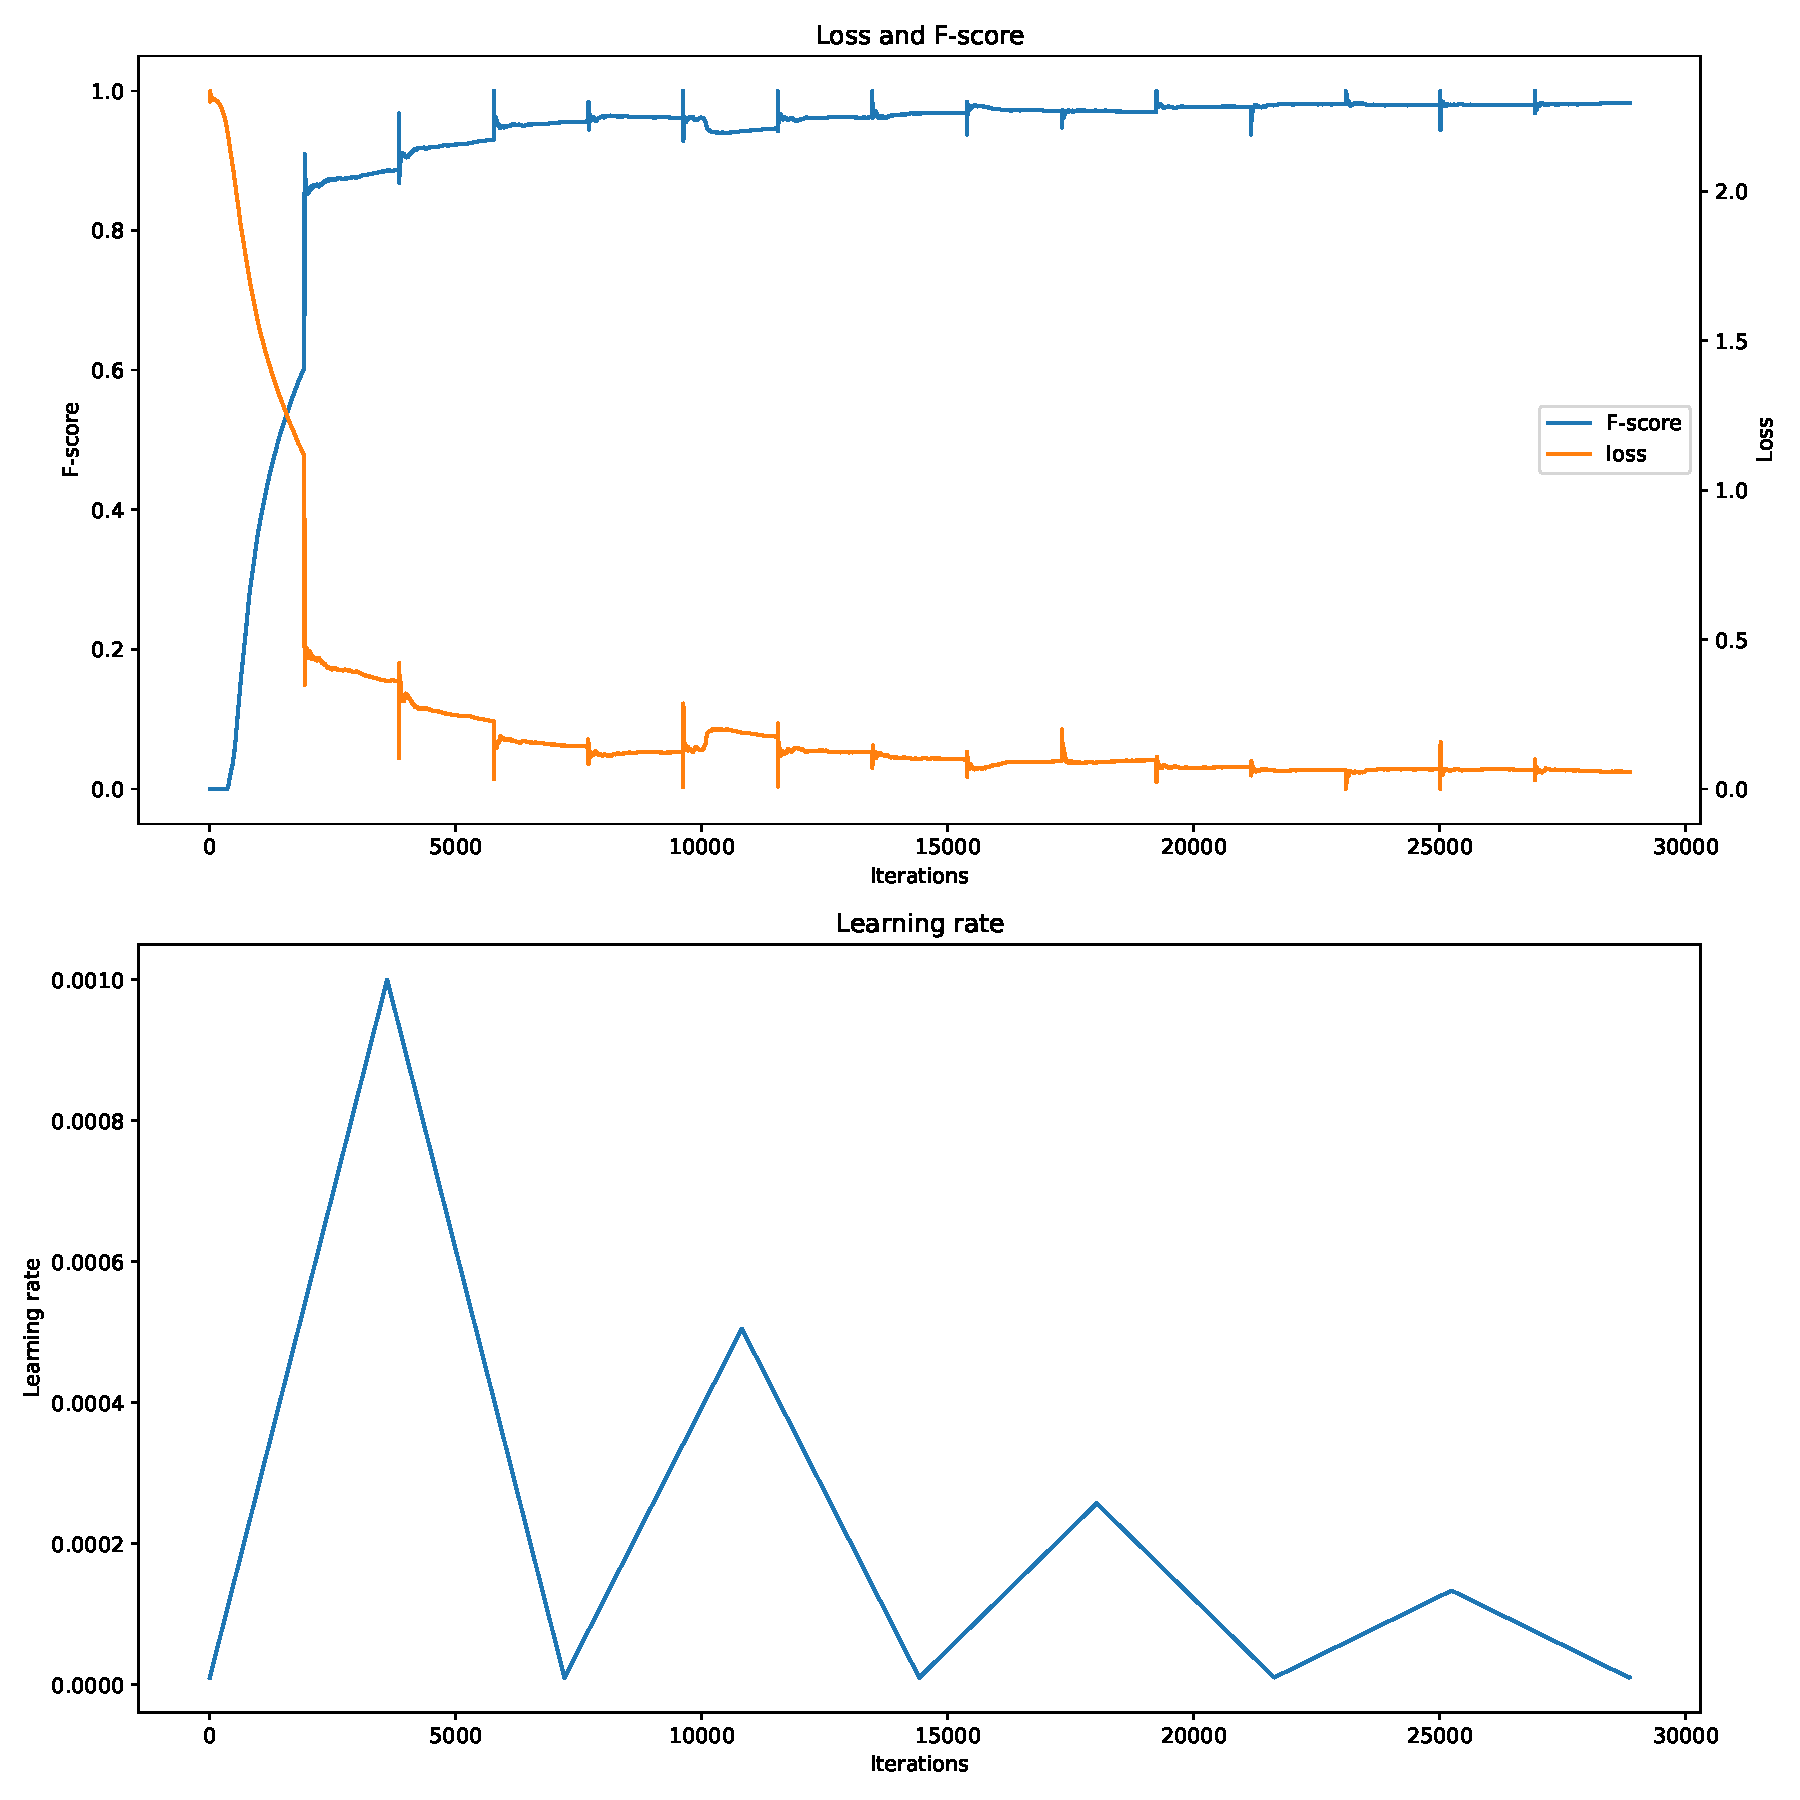
\includegraphics[width=0.9\linewidth]{ATT_ct02_dr01_ks01_lu01_qt04_dw01_opa1_lr07_bs02_en01_dsmela1_wk1_fscore_loss_clr.pdf}
    \caption{Cyclic learning rate schedule example with $4$ cycles.
    The top plot shows the relative F-score and loss of the model.}%
    \label{fig:cyclic_lr_example}
\end{figure}

\subsection{Regularization and Batch Normalization}
TODO or todont?

\subsection{Early stopping}

A very common problem encountered when training a model is overfitting the
data. After a certain number of training epochs, the model has learned
everything it can from the current data, and starts overfitting the
\textit{noise} in the data, instead of meaningful information.
When trying to use the model to make predictions, the results generalize badly.
To prevent this behaviour, a part of the data is kept separate, in the so
called validation fold, and is used to track the performances of the model on
data that it is not training on.
When the validation loss (or any metric that is being tracked, e.g. categorical
accuracy) starts to increase, the training is stopped.
A patience parameter can be set to train for a certain amount of additional
epochs, hoping that the tracked metric will decrease below the current minimum.
Tensorflow allows for model checkpointing, that neatly implements this
behaviour.
TensorBoard is a tool to visualize various metrics and other useful information
during the training of a model, and can be used to compare different training
runs.
During the experiments, early stopping with patience 4 was used.

TODO: Show a plot

\subsection{Optimizer, epochs number and batch size}
TODO or todont?

Adam \cite{kingma2017adam}.

Epoche/batch, tempo di computazione

In each epoch, every sample in the dataset is seen once.
A batch is a set of samples that is used by the optimizer 
algorithm to TODO.

\subsection{Hyper-parameter tuning}

Hyper-parameter tuning was carried out using the class \texttt{ParameterGrid}
implemented in scikit-learn \cite{scikit-learn}.
The class accepts a dictionary that maps parameter names to a list of possible
parameter values and produces all the possible combinations of those values.

The number of combinations quickly grows to unfeasible levels, so a full grid
search cannot be performed.
During the experiments, a three step search was manually performed.
The parameters were split in two sets:
in the first step, the parameters in the first set were kept to a fixed value,
while the others were allowed to change, thus investigating the effects of the
second set of parameters on the training.
In the second step, the roles were reversed:
Once the best values for the second set of parameters were found, these
parameters were kept fixed and the parameters in the first set were allowed to
change.
In the final step, each parameter was allowed to change between the one or two
best values found for it, to fully investigate a reduced grid.

When analyzing the results, special care has to be taken to be sure that
the grids were completely searched.
As an example, say the learning rate parameter can be set to $1$ or $2$
and the epoch number can be either $5$ or $10$.
After some experiments, it is discovered that a learning rate of $2$
outperforms $1$ consistently.
This conclusion is valid if the entire grid was searched, but can be misleading
if only a part of the grid was covered: it might be the case that the only
combinations searched are $(1, 5)$ and $(2, 10)$.
As such, the increase in performance when using a learning rate of $2$ might be
only due to the epoch number set to $10$, whereas the best combination is the
missing one: $(1, 10)$.
No formal way to check for consistency in the grid was developed,
but some care was taken in being methodical when exploring.

% overshadow

TODO: Usare Pool, MAYBE in conclusion/what I learned section.

% Ovviamente non su tutte le combinazioni
% Pay attention (no pun) to over-representation of the good params.

\subsection{Dataset loading}

% TODO: loading the dataset with AudioGenerator

For the datasets with a single spectrogram, even the 35-words task fits easily
in memory. However, for the stacked 3-channel ``images'' with augmented data
the size can grow to 20 gigabytes, which is inconvenient to load at once.
Considering that the training is done in small batches of samples, loading only
the images needed for the current batch is a reasonable approach.
This behaviour was implemented by subclassing the \texttt{Sequence} tensorflow
class, that provides an interface for loading data as needed in a thread safe
way (i.e. it assures that each sample is loaded once per epoch, even when
loading data from multiple threads).
The guide followed to implement the \texttt{AudioGenerator} is available on 
GitHub \cite{afshineaKDG}.

\section{Convolutional Neural Network}
\label{sec:convolutional_arch}

\subsection{Architecture}

As a starting benchmark, a standard Convolutional Neural Network was implemented.
Three convolutional modules are instantiated, followed by a dense classifier.
Each convolutional module is composed of the convolutional layer, a batch
normalization layer, a max pooling layer and a dropout layer.
The classifier is composed by three dense layers, the last with softmax
activation and a number of units equal to the number of classes to predict.

\subsection{Model hyper-parameters}

When building the model, aside from the number of classes to predict and the
input shape of the spectrogram, five parameters can be set:
\begin{enumerate}
    \item Number of convolutional filters: deeper layers have to learn more
        filters, as the feature maps decrease in width and height after the
        pooling.
    \item Shape of the convolutional filters:
        both square and rectangular filters were tested.
        A vertical rectangular filters (e.g. (5, 1)) emphasizes the
        relationship between mel coefficients within the same time step
    \item Shape of the pooling window: 
        both square and rectangular windows were tested.
        Again, a rectangular filter allows to push into deeper layers more
        information along the time or frequency axis.
    \item Dropout rates after the convolutional modules.
    \item Width of the dense classifier layers.
\end{enumerate}
The possible values for the model hyper-parameters are:
\begin{itemize}
    \item dense\_width = [16, 32, 64, 128]
    \item filters = [10, 20, 32, 64, 128]
    \item dropout = [[0.03, 0.01],  [0.3, 0.1]]
    \item kernel\_size = [[(2,2), (2,2), (2,2)], [(5,1), (3,3), (3,3)]]
    \item pool\_size = [[(2,2), (2,2), (2,2)], [(2,1), (2,2), (2,2)]]
\end{itemize}
TODO:
The possible values for the training hyper-parameters are:
\begin{itemize}
    \item batch\_size = [32, 64, 128]
    \item epoch\_num = [15, 30, 60, 100]
    \item lr = ["fixed01", "fixed02", "fixed03",
        "exp\_decay\_step\_01", "exp\_decay\_smooth\_01",
    "exp\_decay\_smooth\_02"]
\end{itemize}

\section{Transfer Learning Approach}
\label{sec:transfer_learning}

\subsection{Transfer learning}

Transfer learning is a technique where a model developed and trained for a task
is modified slightly and used as a starting point for a different task.
A Convolutional Neural Network can be seen as a feature extractor composed with
a classifier.
The feature extractor is the largest part of the network, consisting in roughly
90\% of the trainable weights.
The idea behind transfer learning is to leverage the knowledge acquired
regarding the first part, extracting meaningful features from an image, and
modifying the latter, re-learning the classifier.
Training these big networks (10-100 millions of parameters) on ImageNet (14
millions of images in 1000 classes) can take from days to over a month even on
supercomputers with dozens of top of the line graphics cards.
Adapting the networks for a new task, on the other hand, is a matter of roughly
half an hour on a single GPU.

As spectrograms can be interpreted as images, starting from an image classifier
makes perfect sense. The three architecture used are
DenseNet
\cite{huang2018densely},
Xception 
\cite{chollet2017xception},
and
EfficientNet
\cite{tan2020efficientnet}.

\subsubsection{Xception structure}

A standard convolutional layer tries to learn 3D filters, with two spatial
dimensions and one channel dimension.
Such a filter has to simultaneously learn spatial correlations and
cross-channel correlations.
The Inception Hypothesis asserts that it would be easier to learn independently
the cross-channel and spatial correlations.
To do so an Inception module first learns cross-channel correlations with 1x1
convolutions, then learns spatial correlations with standard 3x3 and 5x5
convolutions.
The Xception model pushed this hypothesis to the limit, completely decoupling
the mapping of spatial and cross-channel correlations.

\subsubsection{EfficientNet structure}

Scaling a Convolutional Neural Network can lead to increased performance:
adding more layers, more filters of more convolutional modules can make the
model more accurate. On the other hand, a bigger model means slower training
and higher memory consumption to the point of being infeasible to train.
On top of that, often CNN can be over-parametrized: model compression
techniques can trade little accuracy for a great reduction in model size
\cite{han2016deep}.

The EfficientNet authors carefully examine the scaling of a model to obtain the
optimal parameters of width, depth and resolution, proposing a new compound
scaling method, which uses a single compound coefficient to scale the three
parameters in a coordinated way.
% which use a compound coefficient φ to uniformly scales network width, depth,
% and resolution in a principled way we have also developed a new mobile-size
% baseline, called EfficientNet fix φ = 1, assuming twice more resources
% available, and do a small grid search of α, β, we then fix α, β, γ as
% constants and scale up baseline network with different φ

\subsubsection{DenseNet structure}

As a Convolutional Neural Network gets deeper, the information about the inputs
or the gradients can vanish by the time it travels through the network.
Many solutions to this problem are available, and they share a central insight:
short paths are created from early layers to later layers.
This idea is explored to the limit in a DenseNet: all layers with matching feature
map size are connected to maximize information flow.
A layer has as inputs all the feature maps of the preceding blocks and is used
as input to all the subsequent layers.
With this topology, a network with $L$ layers has roughly $L^2$ connections.
% Features are composed by concatenating them.

\subsection{Transfer learning and fine tuning}

The pipeline to train a model using transfer learning is as follows:
\begin{enumerate}
    \item Load a previously trained base model, without the final classifier.
    \item Freeze the base model weights, to avoid destroying the information they
        contain.
    \item Add a classifier on top of the base model.
    \item Train the classifier, using a reasonably high learning rate.
    \item Un-freeze the base model weights.
    \item Train the model again, with a very small learning rate, to fine tune
        the feature extractor to the current dataset.
\end{enumerate}

The first four steps are the transfer learning part, followed by the fine
tuning steps five and six.

\subsection{Model building and hyper-parameters}

The inputs to the pre-trained Xception and EfficientNet models have to be
square images with three channels.
To appropriatley shape the input data, three square spectrograms were stacked
along the depth dimension.
On top of that, to obtain square inputs, two rectangular spectrograms were
concatenated horizontally (e.g. two $\left( 128, 64 \right)$ spectrogams are
composed into one $\left( 128, 128 \right)$), before being stacked.
The inputs also need to be normalized, which can be easily done with a
Normalization layer provided by tensorflow.
It is to note that the inputs should be of higher resolution (e.g. $\left( 299,
299, 3 \right)$ for Xception), whereas the spectrograms used were of size
$\left( 128, 128, 3 \right)$, so some loss of performance can be expected.
The classifier built is composed by a GlobalAveragePooling2D layer, which
averages the values in each feature extracted, followed by some dense layers
(according to the hyper-parameters selected) and finally a softmax layer to
compute the predictions.

TODO: specify which models were used

When building the model, aside from the number of classes to predict and the
input shape of the spectrograms, two parameters can be set:
\begin{enumerate}
    \item Dropout rate after the GlobalAveragePooling2D layer.
    \item Dense width and number of the dense layers in the classifier.
\end{enumerate}
The possible values for the hyper-parameters are:
\begin{itemize}
    \item dropout\_types = [0.2, 0.1, 0]
    \item dense\_width\_types = [[4, 0], [16, 16], [0, 0], [64, 64]]
\end{itemize}
Where a value of $0$ means that the layer is skipped.

\section{Attention Model}
\label{sec:attention_model}

\subsection{Attention architecture}

The key idea behind the Attention mechanism is the assumption that not all of
the data that is available carries the same amount of information.
The attention mechanism allows to focus on few relevant details when presented
with large amount of data.
This approach was used effectively in the field of Neural Machine Translation
by Bahdanau \cite{bahdanau2016neural} and Luong \cite{luong2015effective}, and
to produce image captions with the Show, Attend and Tell approach
\cite{xu2016show}.

In the paper by Douglas et al. \cite{2018arXiv180808929C}, the attention
mechanism is used for speech command recognition.
The ouput shapes of each layers are reported to better track along which axis
the dot multiplications are done.
As a first step, the mel spectrogram
(shape [spec\_len, nMel])
is computed from the input audio
(shape [raw\_len]).
A 2D convolution is performed, only along the time axis to extract local
correlations in the spectrogram
(shape [spec\_len, nMel, n\_filters]).
A final 2D convolution, with just one filter, condenses the information back to
a 2D image
(shape [spec\_len, nMel, 1])
and the last dimension is squeezed away
(shape [spec\_len, nMel]).
Two bidirectional \cite{Schuster1997BidirectionalRN} long short-term memory
\cite{lstm} units are used to capture forward and backward long term
dependencies in the spectrogram
(shape [spec\_len, LSTM\_units*2]).
A LSTM layer reads the input sequence from the first sample to the last. The
bidirectional version reads the sequence both forward, producing the forward
hidden states, and backward, resulting in the sequence of backward hidden
states.
Now the attention mechanism is applied: one of the LSTM output vector is
selected (the choice is not crucial because the vectors should contain
information about long term dependencies) and a dense layer is used to extract
a query vector
(shape [LSTM\_units*2]).
The query vector is used to compute the attention scores, by computing the dot
product between all the LSTM outputs and the query vector along the
\textit{second} axis of the LSTM outputs, that are converted with a softmax
layer in attention weights
(shape [spec\_len]).
These weights are multiplied with the output of the LSTM along the
\textit{first} axis of the LSTM outputs to compute a weighted average of the
LSTM vectors
(shape [LSTM\_units*2]),
which is then fed into a dense classifier
(shape [nClasses]).
In this way, the output vector of the LSTM is not just the final hidden state,
but it is a function of all the hidden states, where the most important states
are given more relevance, according to the attention weights.

This architecture will be referred as LSTM+attention in the following sections.

\subsection{Query style}

Two additional methods to compute the query were developed and tested.
In the first method, from the output of the second LSTM layer, a CNN was used
to extract the query, using several convolutional modules.
In the second method, the query was directly computed from the input
spectrogram, using a CNN.
A third query style tested is regarding the choice of LSTM output vector to
pick to compute the query: instead of the last, the central vector was chosen.

TODO: un grafichetto sarebbe bellissimo

\subsection{Model building and hyper-parameters}

When building the model, aside from the number of classes to predict and the
input shape of the spectrograms, six parameters can be set:
\begin{enumerate}
    \item Number of convolutional filters in the convolutional modules.
    \item Dropout rate after the convolutional modules.
    \item Shape of the convolutional filters:
        both square and rectangular filters were tested.
        A vertical rectangular filters (e.g. (5, 1)) emphasizes the
        relationship between mel coefficients within the same time step
    \item Number of LSTM units.
    \item Query style: either a single output vector from the LSTM or the
        result of a convolutional operation, that takes as input the original
        spectrogam or the vectors produced by the LSTM.
    \item Width of the dense classifier layers.
\end{enumerate}
The possible values for the hyper-parameters are:
\begin{itemize}
    \item conv\_size = [[10, 0, 1], [10, 10, 1]]
    \item dropout = {0.2, 0}
    \item kernel\_size = [[(5,1), (5,1), (5,1)], [(3,3), (3,3), (3,3)]]
    \item lstm\_units = [[64, 64], [64, 0]]
    \item query\_style = ["dense01", "dense02", "conv01", "conv02", "conv03"]
    \item dense\_width = [32, 64]
\end{itemize}

TODO: hyper-parameter for training (e.g. lr)

\section{SimpleNet, AreaNet and VerticalAreaNet}
% Dream a dream

\subsubsection{SimpleNet}

While developing the AreaNet architecture, a regular convolutional neural
network was used to extract the attention scores and classify the weighted
inputs.
Due to an error in the first implementation of the softmax layer, the weights
used were all equal to one, cutting off the key part of the network that was
used to apply the attention mechanism.
However, the classifier achieved a very good performance even without weighing
the input, so it was upgraded from being just a building block of the AreaNet
to one of the proposed solutions to the problem, and referenced as SimpleNet.

The main difference with the convolutional architechture proposed in
\secref{sec:convolutional_arch} is in the classifier structure:
instead of flattening the last feature maps obtained
(shape $(batch\_size, height, width, num\_filters)$),
a GlobalAvgPool2D layer was used.
This layer computes the mean in every feature map, obtaining a single value per
map (shape $(batch\_size, num\_filters)$).
These values are directly connected to a Dense layer used to predict the classes,
using a softmax activation layer.

\subsubsection{AreaNet and VerticalAreaNet}

The driving idea behind AreaNet and VerticalAreaNet is to score the original
spectrogram image with a grid of attention scores.
AreaNet builds a $8 \times 8$ grid to weigh the input data,
(\fig{fig:attention_weights_area}),
while
VerticalAreaNet builds a $1 \times 16$ grid to weigh the input data,
(\fig{fig:attention_weights_vertical}).
By using a one dimensional grid, VerticalAreaNet only weighs the input along
the time axis.

To compute the grid weights, the input image is fed into a convolutional network,
that includes several MaxPooling layers that downsample the feature maps generated.
For AreaNet, in the last layer of the weight extractor the mean along the depth
axis is computed to reduce the $num\_filter$ feature maps to a single image,
then the scores are converted into a valid probability distribution using a
softmax activation function, and finally the weights are upsampled back to the
original shape of the input.
For VerticalAreaNet, the mean is also computed along the time axis to obtain
a one dimensional vector, that is then upsampled.

For both architectures, the weighted spectrogram is then used as input for a
SimpleNet, used to classify the audio sample.

\begin{figure}[t!]
    \centering
    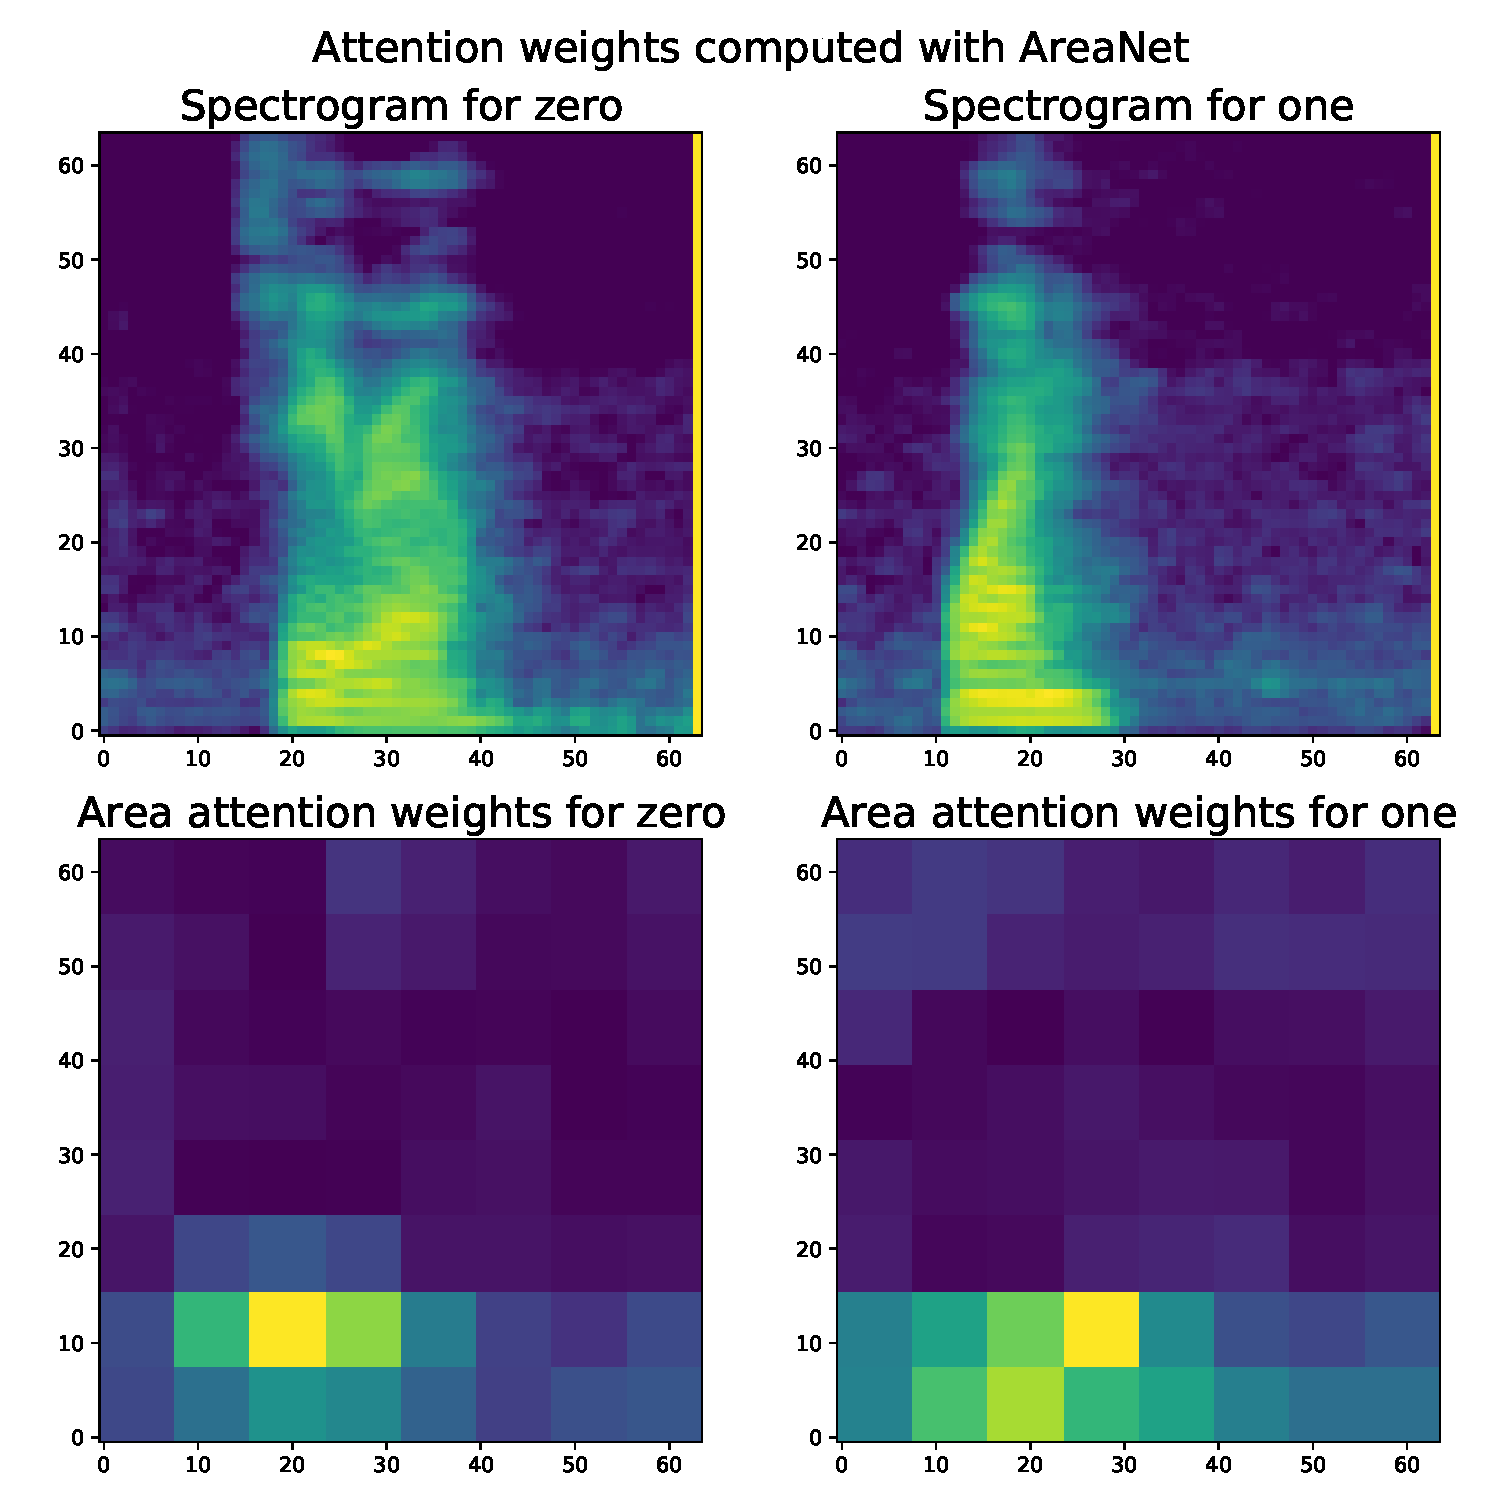
\includegraphics[width=0.9\linewidth]{AAN_opa1_lr03_bs32_en15_dsaug14_wLTnum_0001.pdf}
    \caption{AreaNet computes a $8 \times 8$ grid that is used to weigh the
    original spectrogram.
    It can be seen that the model focuses on the lowest frequencies aligned
    with the portion of utterance where the word is actually being spoken,
    correctly extracting the relevant portion of the spectrograms. }%
    \label{fig:attention_weights_area}
\end{figure}

\begin{figure}[t!]
    \centering
    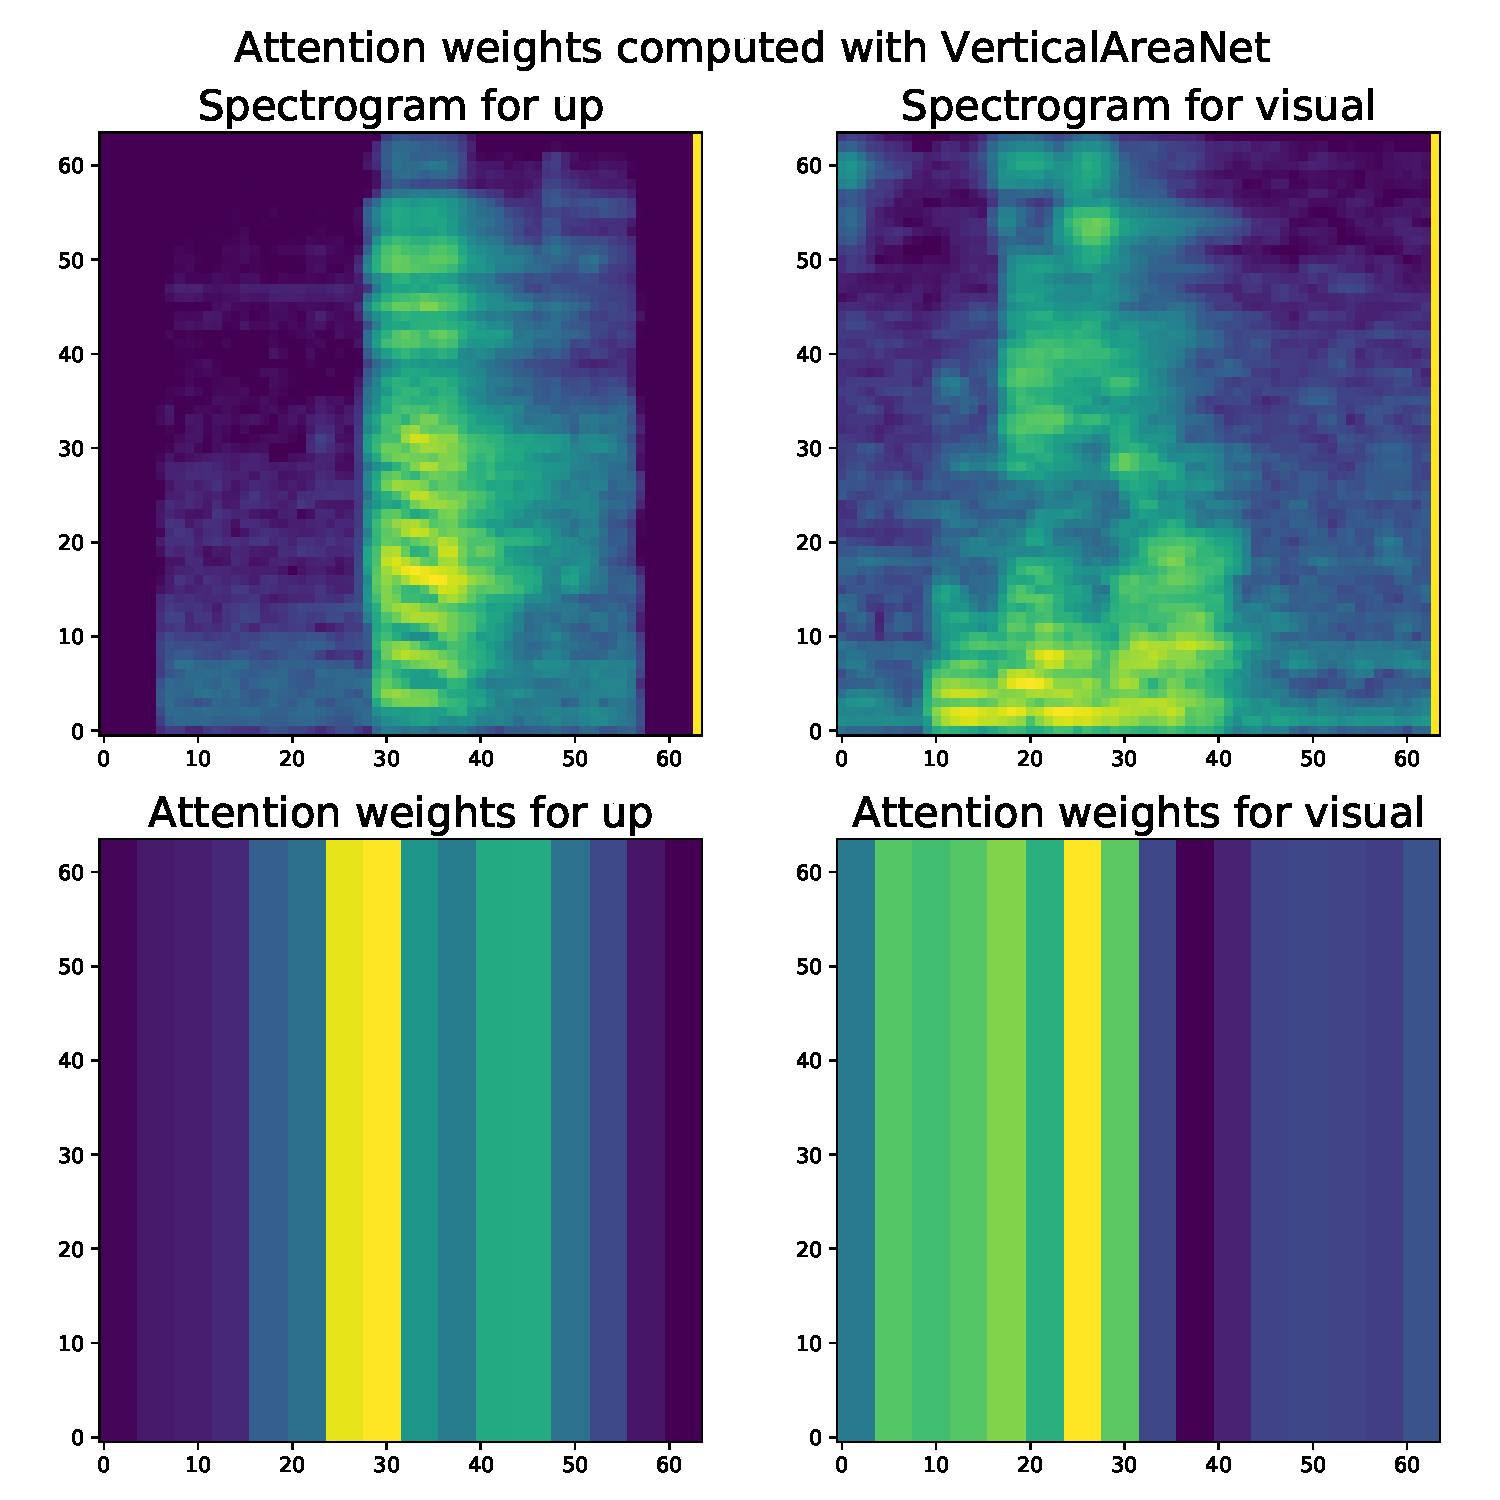
\includegraphics[width=0.9\linewidth]{VAN_opa1_lr04_bs32_en15_dsaug14_wLTall_0001.pdf}
    \caption{VerticalAreaNet computes a $1 \times 16$ grid that is used to
        weigh the original 
    spectrogram.}%
    \label{fig:attention_weights_vertical}
\end{figure}
